%!TEX program = pdflatex
\documentclass[lang=cn]{elegantpaper}
\title{Matlb-GUI编程}
\author{何长鸿-2016141482154}
\date{\today}
\begin{document}
\maketitle

%%%%%%%%%%%%%%%%%%%%%%%%%%%%%%%%%
\section{初始图像及参数界面}
\par 界面编辑如图 \ref{fig:img0},默认读入图片显示在inputImg标签,如图\ref{fig:img1}
    \begin{figure}[htbp]
        \centering
        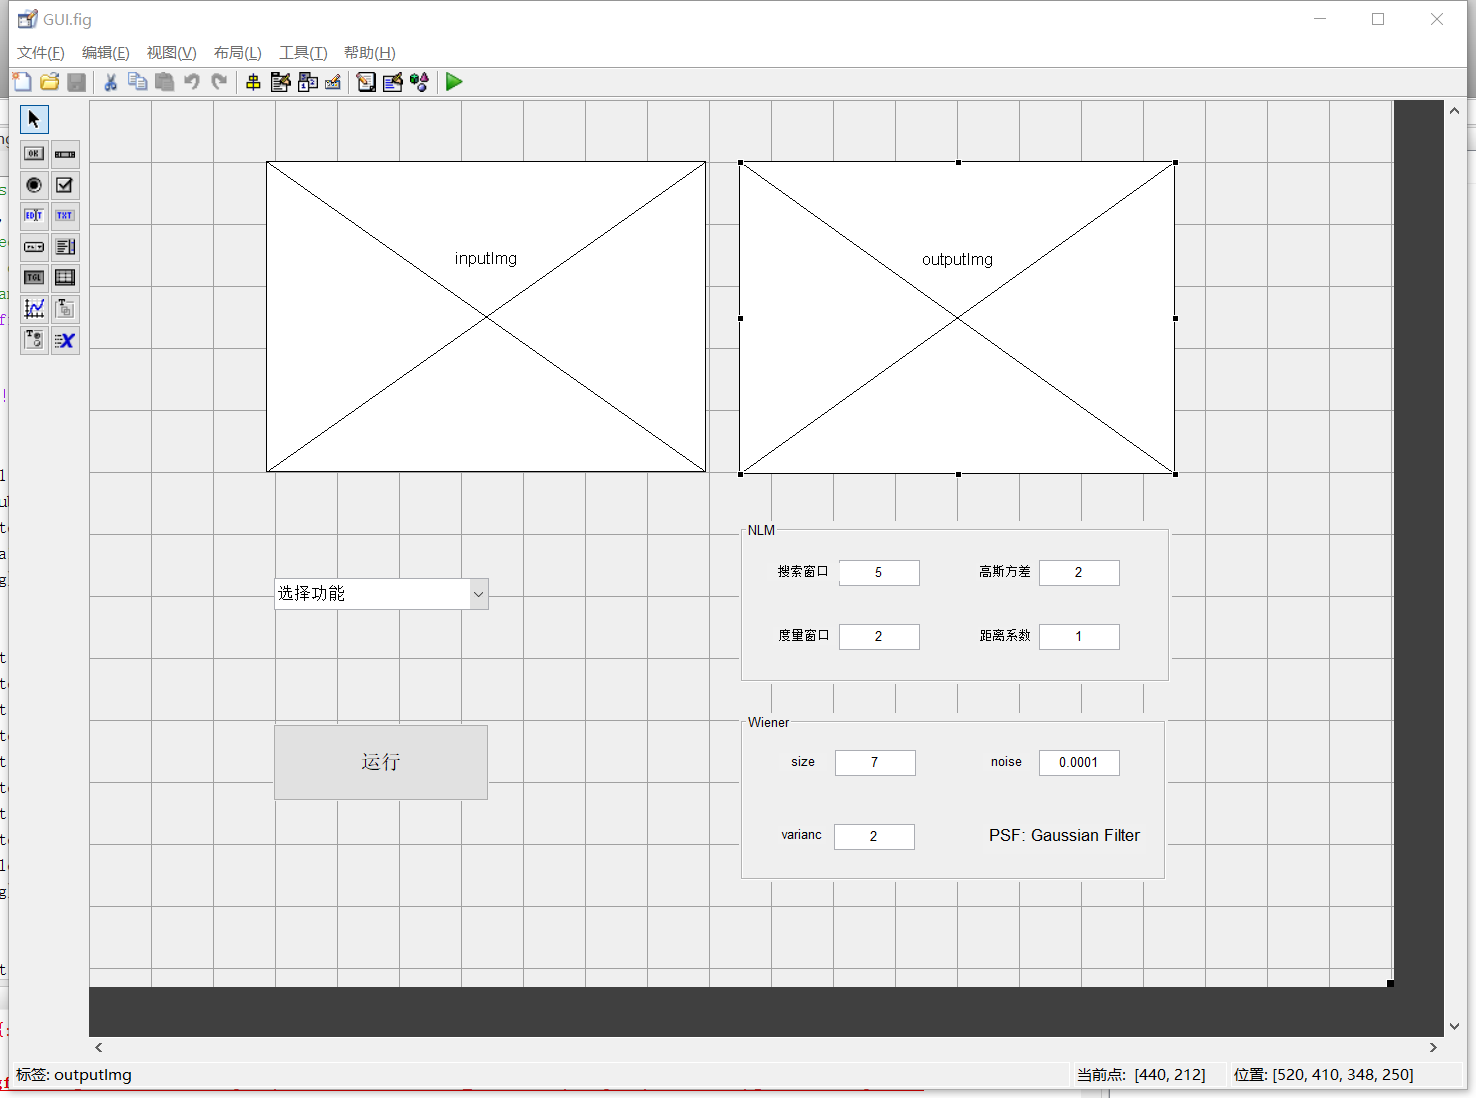
\includegraphics[width=0.6\textwidth]{img0.png}
        \caption{fig编辑界面\label{fig:img0}}
        
        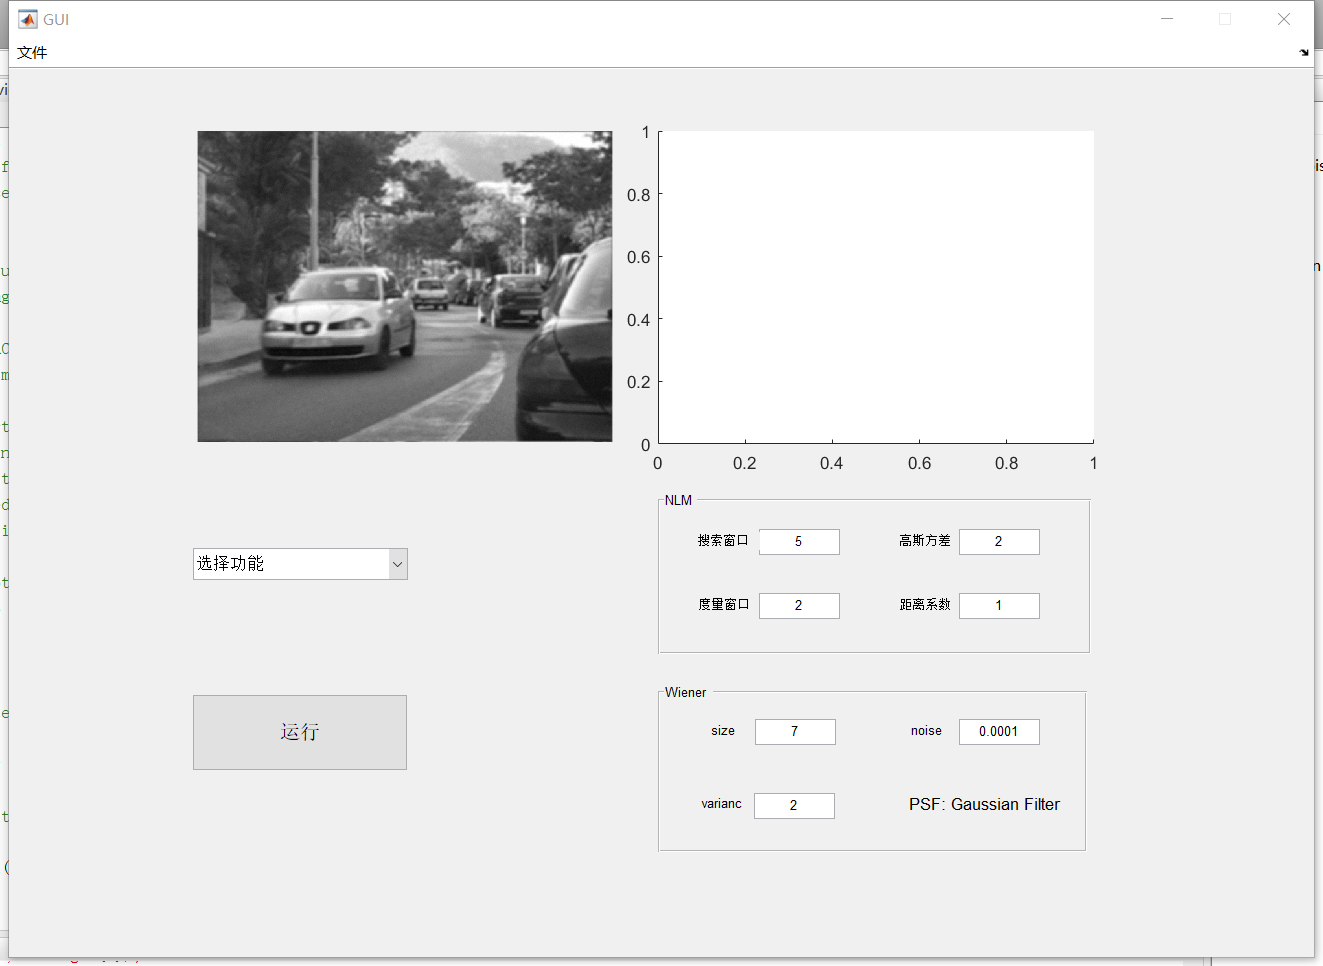
\includegraphics[width=0.6\textwidth]{img1.png}
        \caption{fig编辑界面\label{fig:img1}}
    \end{figure}
%%%%%%%%%%%%%%%%%%%%%%%%%%%%%%%%%%
\section{菜单栏打开图像}
\par 添加通过菜单选择并打开本地图像,并显示,如图\ref{fig:img2}、\ref{fig:img3}
    \begin{figure}[htbp]
        \centering
        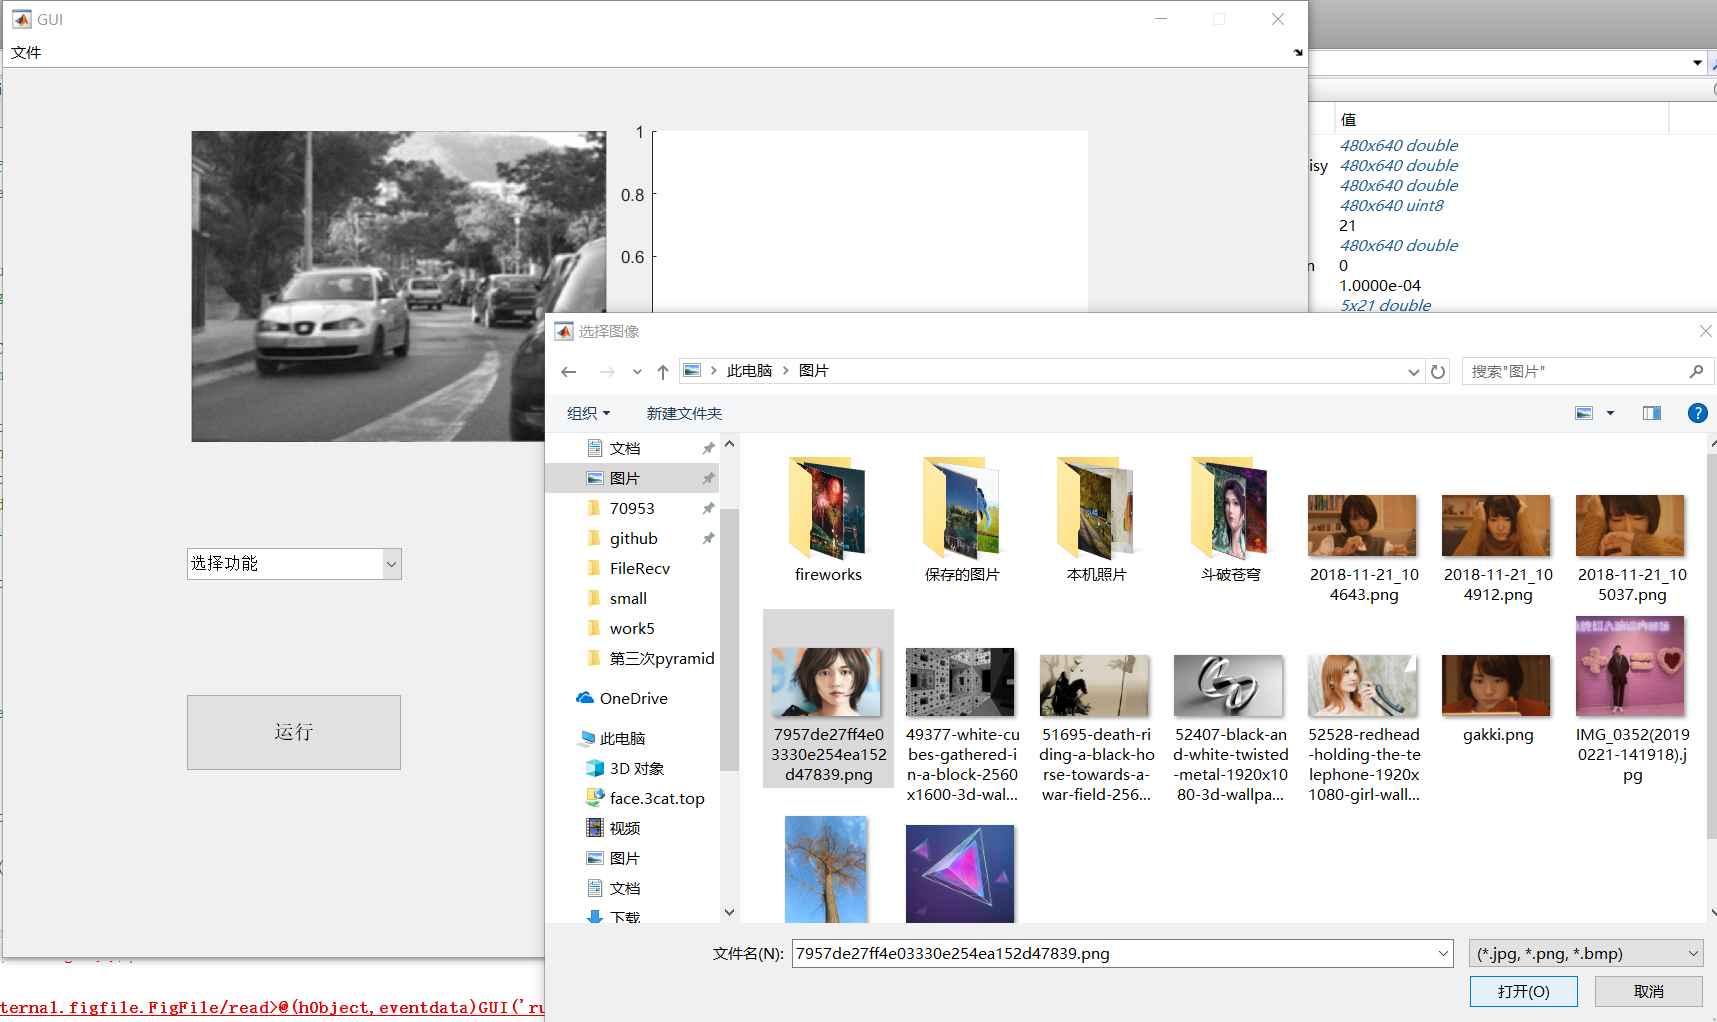
\includegraphics[width=0.6\textwidth]{img2.png}
        \caption{fig编辑界面\label{fig:img2}}
        
        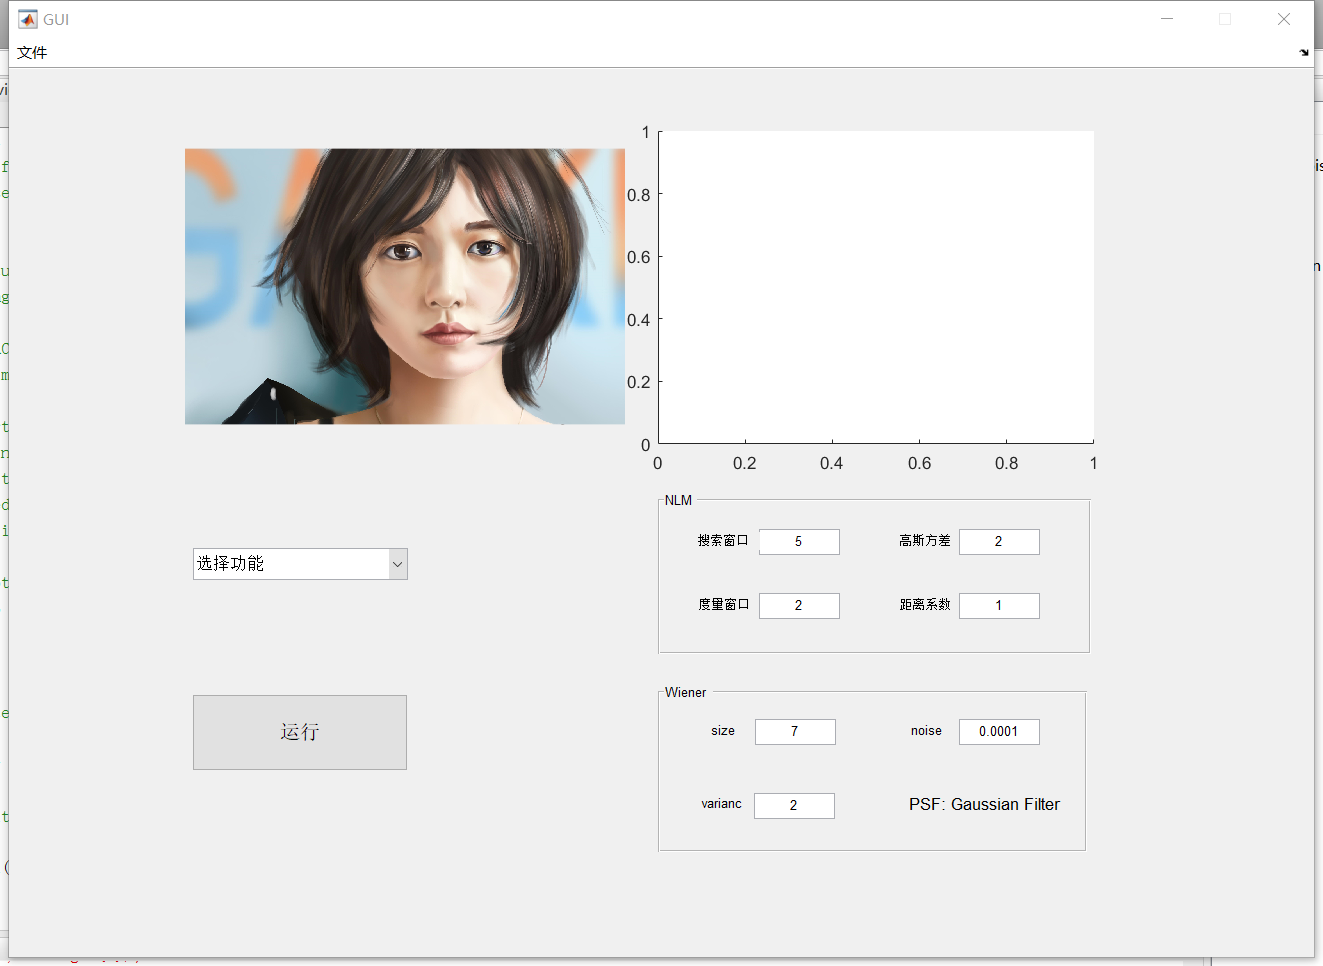
\includegraphics[width=0.6\textwidth]{img3.png}
        \caption{fig编辑界面\label{fig:img3}}
    \end{figure}

\section{控制编辑框状态}
\par 若选择“图像增强”,则所有可输入文本框变灰;若选择“图像去噪”,与去噪不相关的输入文本框变灰;若选择“图像复原”,与复原无关的输入系数文本框变灰,
如图\ref{fig:img4}
\begin{figure}[htbp]
    \centering
    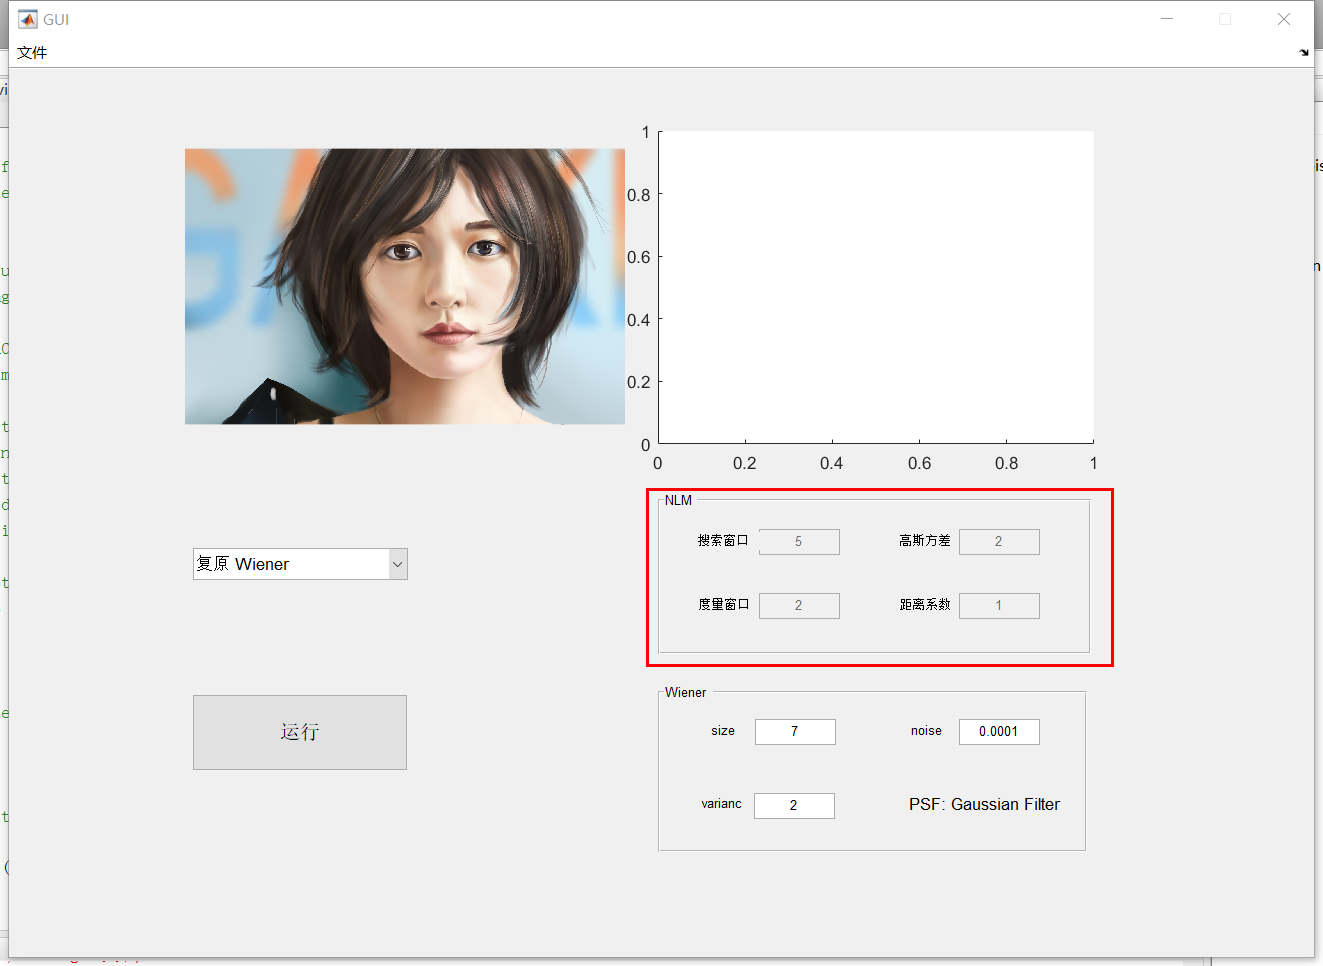
\includegraphics[width=0.6\textwidth]{img4.png}
    \caption{fig编辑界面\label{fig:img4}}
\end{figure}

\section{图像增强、去噪、恢复}
\par 图像增强效果如图\ref{fig:img5}
    \begin{figure}[htbp]
        \centering
        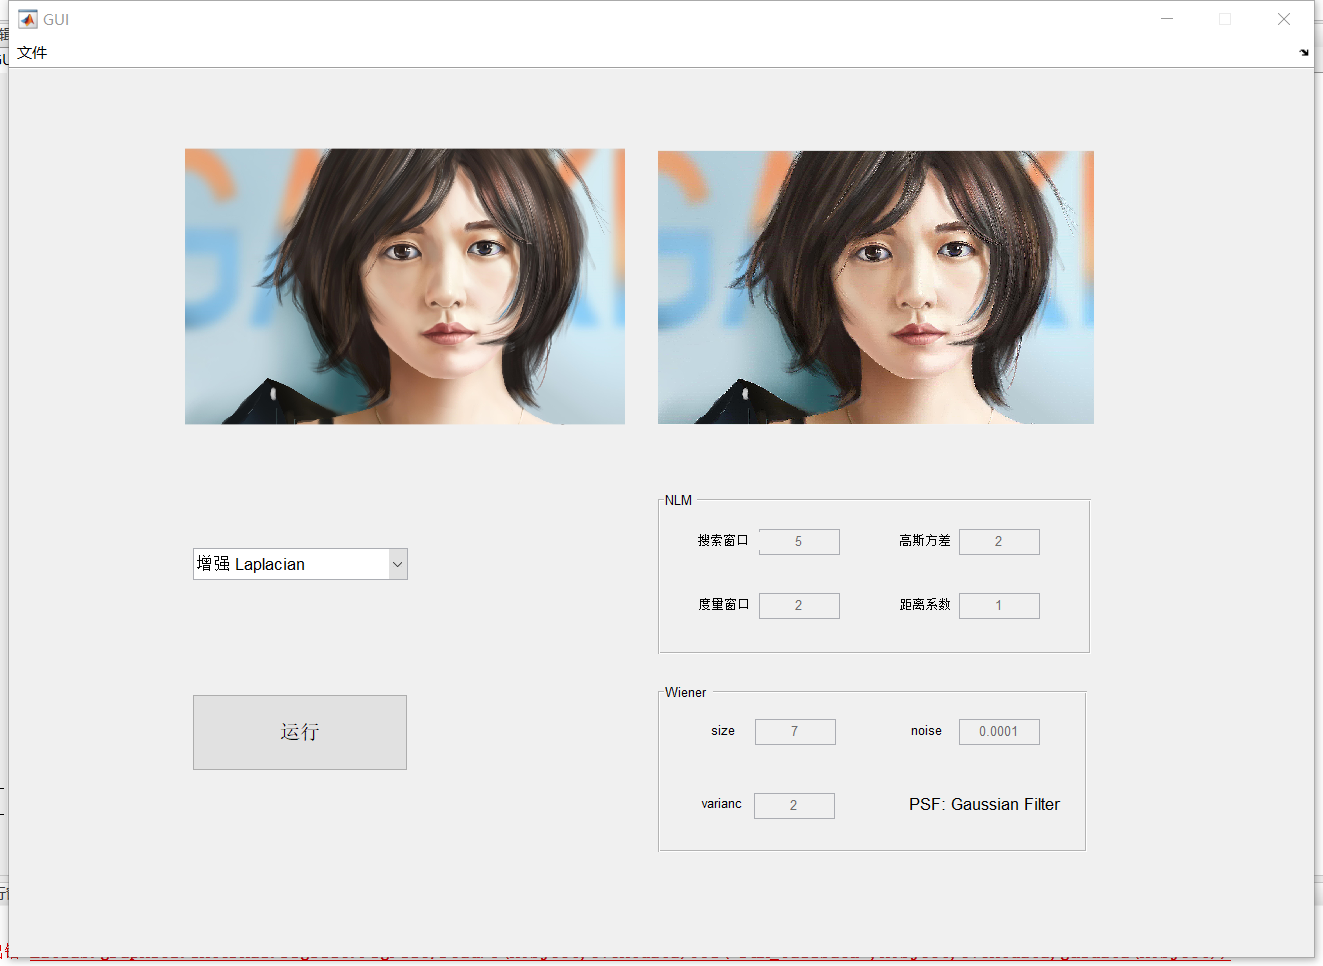
\includegraphics[width=0.6\textwidth]{img5.png}
        \caption{fig编辑界面\label{fig:img5}}
    \end{figure}

\par 图像NLM去噪,使用第二章的噪点图片,去噪效果和对应参数如图\ref{fig:img6}
    \begin{figure}[htbp]
        \centering
        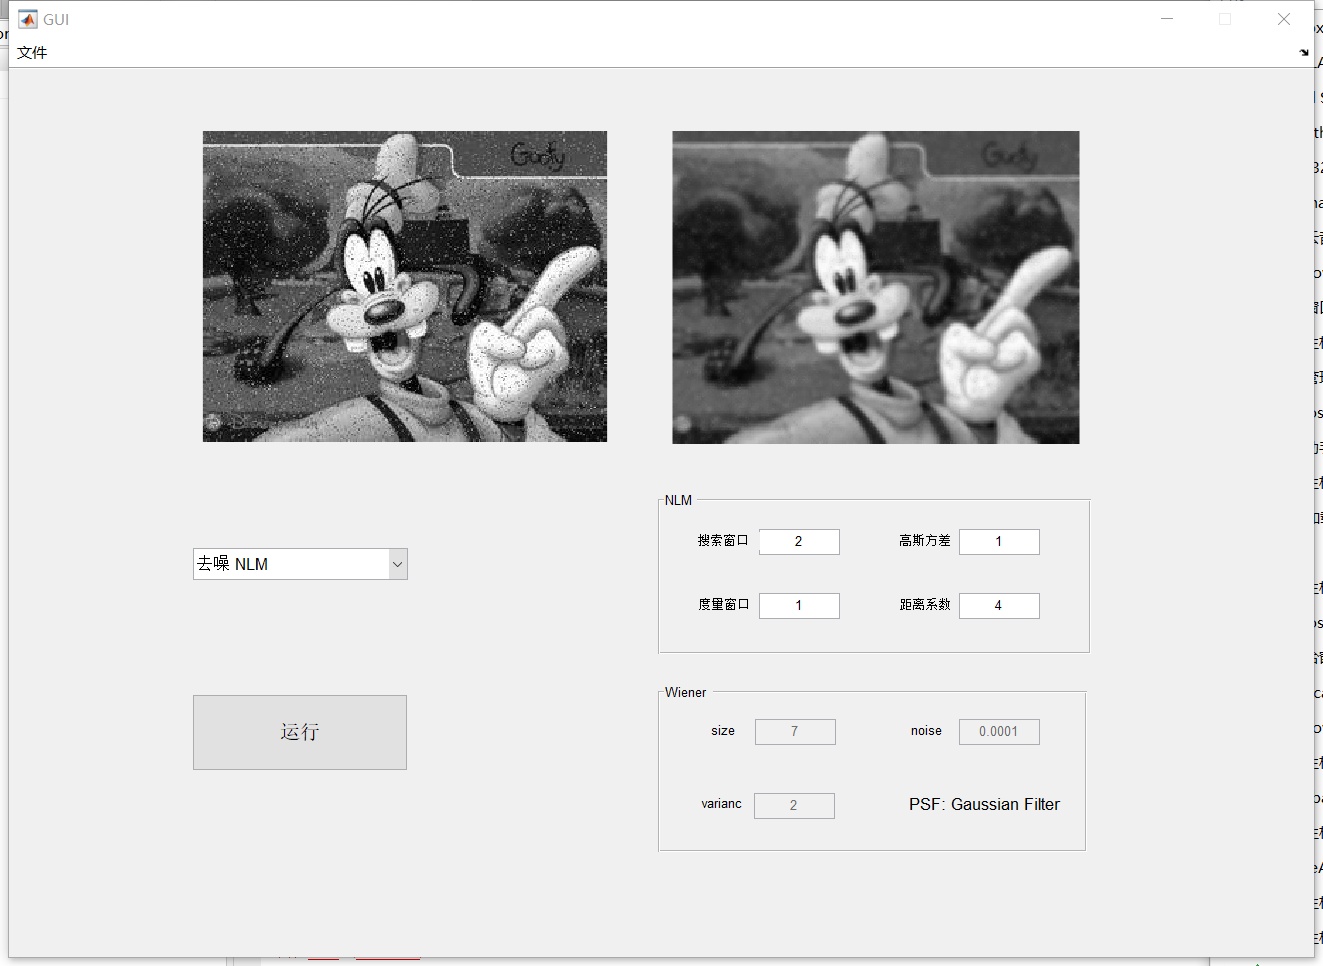
\includegraphics[width=0.6\textwidth]{img6.png}
        \caption{fig编辑界面\label{fig:img6}}
    \end{figure}

\par 图像Wiener,先对本章给定的ingputImg.bmp进行模糊以及加入噪声处理,得到输入图像,再对其进行Wiener恢复,效果如图\ref{fig:img7}
    \begin{figure}[htbp]
        \centering
        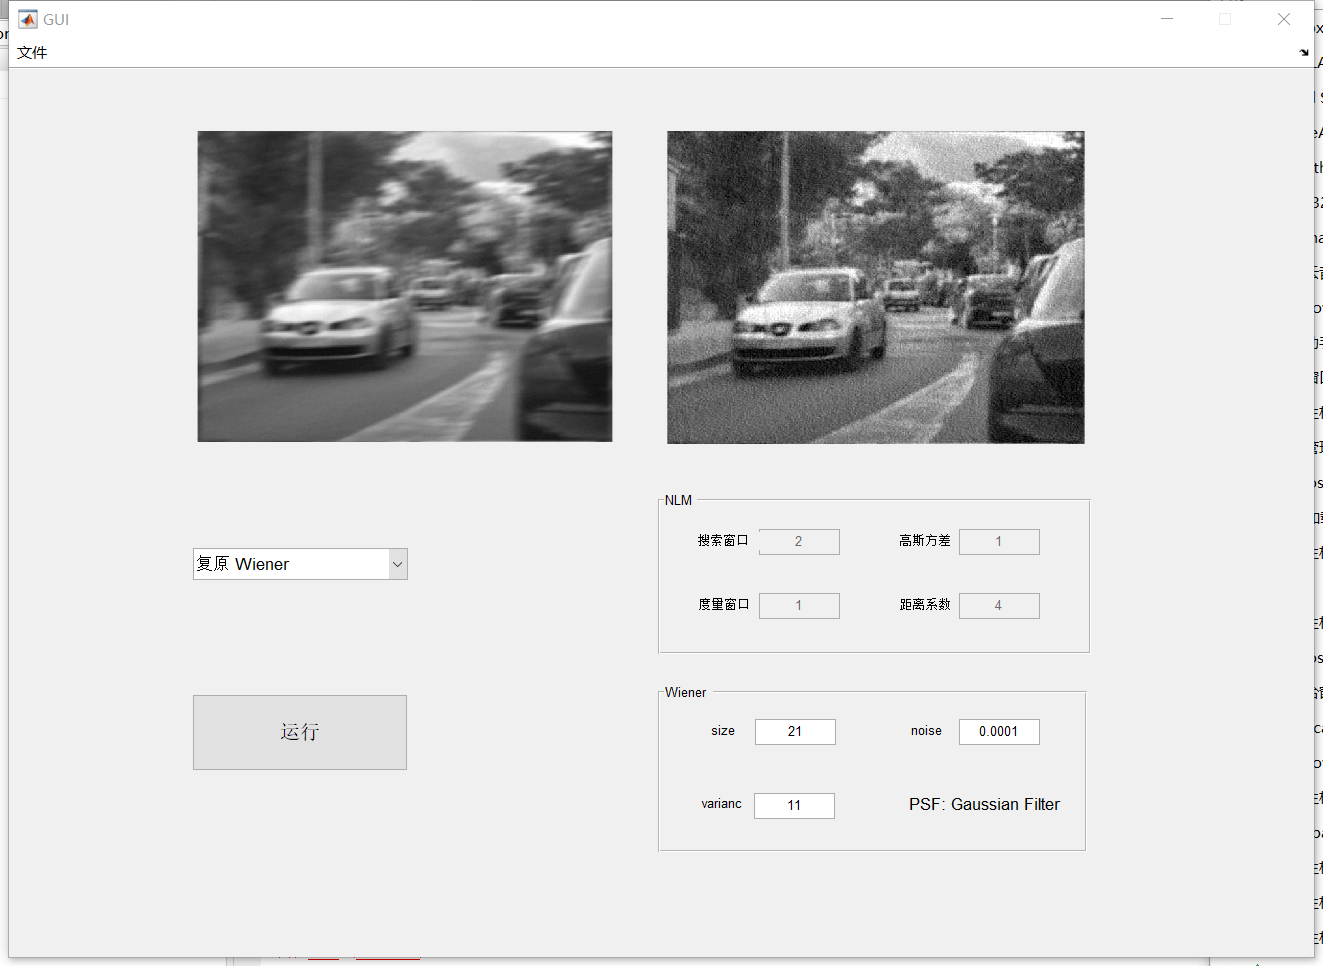
\includegraphics[width=0.6\textwidth]{img7.png}
        \caption{fig编辑界面\label{fig:img7}}
    \end{figure}
\end{document}
